\documentclass[border=1in]{standalone}

    \usepackage[breakable]{tcolorbox}
    \usepackage{parskip} % Stop auto-indenting (to mimic markdown behaviour)
    \usepackage{subfiles}
    \usepackage{iftex}
	 \ifPDFTeX
    	\usepackage[T1]{fontenc}
    	\usepackage{mathpazo}
    \else
    	\usepackage{fontspec}
    \fi

    % Basic figure setup, for now with no caption control since it's done
    % automatically by Pandoc (which extracts ![](path) syntax from Markdown).
    \usepackage{graphicx}
    % Maintain compatibility with old templates. Remove in nbconvert 6.0
    \let\Oldincludegraphics\includegraphics
    % Ensure that by default, figures have no caption (until we provide a
    % proper Figure object with a Caption API and a way to capture that
    % in the conversion process - todo).
    \usepackage{caption}
    \DeclareCaptionFormat{nocaption}{}
    \captionsetup{format=nocaption,aboveskip=0pt,belowskip=0pt}

    \usepackage{float}
    \floatplacement{figure}{H} % forces figures to be placed at the correct location
    \usepackage{xcolor} % Allow colors to be defined
    \usepackage{enumerate} % Needed for markdown enumerations to work
    \usepackage{geometry} % Used to adjust the document margins
    \usepackage{amsmath} % Equations
    \usepackage{amssymb} % Equations
    \usepackage{textcomp} % defines textquotesingle
    % Hack from http://tex.stackexchange.com/a/47451/13684:
    \AtBeginDocument{%
        \def\PYZsq{\textquotesingle}% Upright quotes in Pygmentized code
    }
    \usepackage{upquote} % Upright quotes for verbatim code
    \usepackage{eurosym} % defines \euro
    \usepackage[mathletters]{ucs} % Extended unicode (utf-8) support
    \usepackage{fancyvrb} % verbatim replacement that allows latex
    \usepackage{grffile} % extends the file name processing of package graphics 
                         % to support a larger range
    \makeatletter % fix for old versions of grffile with XeLaTeX
    \@ifpackagelater{grffile}{2019/11/01}
    {
      % Do nothing on new versions
    }
    {
      \def\Gread@@xetex#1{%
        \IfFileExists{"\Gin@base".bb}%
        {\Gread@eps{\Gin@base.bb}}%
        {\Gread@@xetex@aux#1}%
      }
    }
    \makeatother
    \usepackage[Export]{adjustbox} % Used to constrain images to a maximum size
    \adjustboxset{max size={0.9\linewidth}{0.9\paperheight}}

    % The hyperref package gives us a pdf with properly built
    % internal navigation ('pdf bookmarks' for the table of contents,
    % internal cross-reference links, web links for URLs, etc.)
    \usepackage{hyperref}
    % The default LaTeX title has an obnoxious amount of whitespace. By default,
    % titling removes some of it. It also provides customization options.
    \usepackage{titling}
    \usepackage{longtable} % longtable support required by pandoc >1.10
    \usepackage{booktabs}  % table support for pandoc > 1.12.2
    \usepackage[inline]{enumitem} % IRkernel/repr support (it uses the enumerate* environment)
    \usepackage[normalem]{ulem} % ulem is needed to support strikethroughs (\sout)
                                % normalem makes italics be italics, not underlines
    \usepackage{mathrsfs}
    

    
    % Colors for the hyperref package
    \definecolor{urlcolor}{rgb}{0,.145,.698}
    \definecolor{linkcolor}{rgb}{.71,0.21,0.01}
    \definecolor{citecolor}{rgb}{.12,.54,.11}

    % ANSI colors
    \definecolor{ansi-black}{HTML}{3E424D}
    \definecolor{ansi-black-intense}{HTML}{282C36}
    \definecolor{ansi-red}{HTML}{E75C58}
    \definecolor{ansi-red-intense}{HTML}{B22B31}
    \definecolor{ansi-green}{HTML}{00A250}
    \definecolor{ansi-green-intense}{HTML}{007427}
    \definecolor{ansi-yellow}{HTML}{DDB62B}
    \definecolor{ansi-yellow-intense}{HTML}{B27D12}
    \definecolor{ansi-blue}{HTML}{208FFB}
    \definecolor{ansi-blue-intense}{HTML}{0065CA}
    \definecolor{ansi-magenta}{HTML}{D160C4}
    \definecolor{ansi-magenta-intense}{HTML}{A03196}
    \definecolor{ansi-cyan}{HTML}{60C6C8}
    \definecolor{ansi-cyan-intense}{HTML}{258F8F}
    \definecolor{ansi-white}{HTML}{C5C1B4}
    \definecolor{ansi-white-intense}{HTML}{A1A6B2}
    \definecolor{ansi-default-inverse-fg}{HTML}{FFFFFF}
    \definecolor{ansi-default-inverse-bg}{HTML}{000000}

    % common color for the border for error outputs.
    \definecolor{outerrorbackground}{HTML}{FFDFDF}

    % commands and environments needed by pandoc snippets
    % extracted from the output of `pandoc -s`
    \providecommand{\tightlist}{%
      \setlength{\itemsep}{0pt}\setlength{\parskip}{0pt}}
    \DefineVerbatimEnvironment{Highlighting}{Verbatim}{commandchars=\\\{\}}
    % Add ',fontsize=\small' for more characters per line
    \newenvironment{Shaded}{}{}
    \newcommand{\KeywordTok}[1]{\textcolor[rgb]{0.00,0.44,0.13}{\textbf{{#1}}}}
    \newcommand{\DataTypeTok}[1]{\textcolor[rgb]{0.56,0.13,0.00}{{#1}}}
    \newcommand{\DecValTok}[1]{\textcolor[rgb]{0.25,0.63,0.44}{{#1}}}
    \newcommand{\BaseNTok}[1]{\textcolor[rgb]{0.25,0.63,0.44}{{#1}}}
    \newcommand{\FloatTok}[1]{\textcolor[rgb]{0.25,0.63,0.44}{{#1}}}
    \newcommand{\CharTok}[1]{\textcolor[rgb]{0.25,0.44,0.63}{{#1}}}
    \newcommand{\StringTok}[1]{\textcolor[rgb]{0.25,0.44,0.63}{{#1}}}
    \newcommand{\CommentTok}[1]{\textcolor[rgb]{0.38,0.63,0.69}{\textit{{#1}}}}
    \newcommand{\OtherTok}[1]{\textcolor[rgb]{0.00,0.44,0.13}{{#1}}}
    \newcommand{\AlertTok}[1]{\textcolor[rgb]{1.00,0.00,0.00}{\textbf{{#1}}}}
    \newcommand{\FunctionTok}[1]{\textcolor[rgb]{0.02,0.16,0.49}{{#1}}}
    \newcommand{\RegionMarkerTok}[1]{{#1}}
    \newcommand{\ErrorTok}[1]{\textcolor[rgb]{1.00,0.00,0.00}{\textbf{{#1}}}}
    \newcommand{\NormalTok}[1]{{#1}}
    
    % Additional commands for more recent versions of Pandoc
    \newcommand{\ConstantTok}[1]{\textcolor[rgb]{0.53,0.00,0.00}{{#1}}}
    \newcommand{\SpecialCharTok}[1]{\textcolor[rgb]{0.25,0.44,0.63}{{#1}}}
    \newcommand{\VerbatimStringTok}[1]{\textcolor[rgb]{0.25,0.44,0.63}{{#1}}}
    \newcommand{\SpecialStringTok}[1]{\textcolor[rgb]{0.73,0.40,0.53}{{#1}}}
    \newcommand{\ImportTok}[1]{{#1}}
    \newcommand{\DocumentationTok}[1]{\textcolor[rgb]{0.73,0.13,0.13}{\textit{{#1}}}}
    \newcommand{\AnnotationTok}[1]{\textcolor[rgb]{0.38,0.63,0.69}{\textbf{\textit{{#1}}}}}
    \newcommand{\CommentVarTok}[1]{\textcolor[rgb]{0.38,0.63,0.69}{\textbf{\textit{{#1}}}}}
    \newcommand{\VariableTok}[1]{\textcolor[rgb]{0.10,0.09,0.49}{{#1}}}
    \newcommand{\ControlFlowTok}[1]{\textcolor[rgb]{0.00,0.44,0.13}{\textbf{{#1}}}}
    \newcommand{\OperatorTok}[1]{\textcolor[rgb]{0.40,0.40,0.40}{{#1}}}
    \newcommand{\BuiltInTok}[1]{{#1}}
    \newcommand{\ExtensionTok}[1]{{#1}}
    \newcommand{\PreprocessorTok}[1]{\textcolor[rgb]{0.74,0.48,0.00}{{#1}}}
    \newcommand{\AttributeTok}[1]{\textcolor[rgb]{0.49,0.56,0.16}{{#1}}}
    \newcommand{\InformationTok}[1]{\textcolor[rgb]{0.38,0.63,0.69}{\textbf{\textit{{#1}}}}}
    \newcommand{\WarningTok}[1]{\textcolor[rgb]{0.38,0.63,0.69}{\textbf{\textit{{#1}}}}}
    
    
    % Define a nice break command that doesn't care if a line doesn't already
    % exist.
    \def\br{\hspace*{\fill} \\* }
    % Math Jax compatibility definitions
    \def\gt{>}
    \def\lt{<}
    \let\Oldtex\TeX
    \let\Oldlatex\LaTeX
    \renewcommand{\TeX}{\textrm{\Oldtex}}
    \renewcommand{\LaTeX}{\textrm{\Oldlatex}}
    % Document parameters
    % Document title
    \title{LABexc2-ELE510-2021}
    
    
    
    
    
% Pygments definitions
\makeatletter
\def\PY@reset{\let\PY@it=\relax \let\PY@bf=\relax%
    \let\PY@ul=\relax \let\PY@tc=\relax%
    \let\PY@bc=\relax \let\PY@ff=\relax}
\def\PY@tok#1{\csname PY@tok@#1\endcsname}
\def\PY@toks#1+{\ifx\relax#1\empty\else%
    \PY@tok{#1}\expandafter\PY@toks\fi}
\def\PY@do#1{\PY@bc{\PY@tc{\PY@ul{%
    \PY@it{\PY@bf{\PY@ff{#1}}}}}}}
\def\PY#1#2{\PY@reset\PY@toks#1+\relax+\PY@do{#2}}

\expandafter\def\csname PY@tok@w\endcsname{\def\PY@tc##1{\textcolor[rgb]{0.73,0.73,0.73}{##1}}}
\expandafter\def\csname PY@tok@c\endcsname{\let\PY@it=\textit\def\PY@tc##1{\textcolor[rgb]{0.25,0.50,0.50}{##1}}}
\expandafter\def\csname PY@tok@cp\endcsname{\def\PY@tc##1{\textcolor[rgb]{0.74,0.48,0.00}{##1}}}
\expandafter\def\csname PY@tok@k\endcsname{\let\PY@bf=\textbf\def\PY@tc##1{\textcolor[rgb]{0.00,0.50,0.00}{##1}}}
\expandafter\def\csname PY@tok@kp\endcsname{\def\PY@tc##1{\textcolor[rgb]{0.00,0.50,0.00}{##1}}}
\expandafter\def\csname PY@tok@kt\endcsname{\def\PY@tc##1{\textcolor[rgb]{0.69,0.00,0.25}{##1}}}
\expandafter\def\csname PY@tok@o\endcsname{\def\PY@tc##1{\textcolor[rgb]{0.40,0.40,0.40}{##1}}}
\expandafter\def\csname PY@tok@ow\endcsname{\let\PY@bf=\textbf\def\PY@tc##1{\textcolor[rgb]{0.67,0.13,1.00}{##1}}}
\expandafter\def\csname PY@tok@nb\endcsname{\def\PY@tc##1{\textcolor[rgb]{0.00,0.50,0.00}{##1}}}
\expandafter\def\csname PY@tok@nf\endcsname{\def\PY@tc##1{\textcolor[rgb]{0.00,0.00,1.00}{##1}}}
\expandafter\def\csname PY@tok@nc\endcsname{\let\PY@bf=\textbf\def\PY@tc##1{\textcolor[rgb]{0.00,0.00,1.00}{##1}}}
\expandafter\def\csname PY@tok@nn\endcsname{\let\PY@bf=\textbf\def\PY@tc##1{\textcolor[rgb]{0.00,0.00,1.00}{##1}}}
\expandafter\def\csname PY@tok@ne\endcsname{\let\PY@bf=\textbf\def\PY@tc##1{\textcolor[rgb]{0.82,0.25,0.23}{##1}}}
\expandafter\def\csname PY@tok@nv\endcsname{\def\PY@tc##1{\textcolor[rgb]{0.10,0.09,0.49}{##1}}}
\expandafter\def\csname PY@tok@no\endcsname{\def\PY@tc##1{\textcolor[rgb]{0.53,0.00,0.00}{##1}}}
\expandafter\def\csname PY@tok@nl\endcsname{\def\PY@tc##1{\textcolor[rgb]{0.63,0.63,0.00}{##1}}}
\expandafter\def\csname PY@tok@ni\endcsname{\let\PY@bf=\textbf\def\PY@tc##1{\textcolor[rgb]{0.60,0.60,0.60}{##1}}}
\expandafter\def\csname PY@tok@na\endcsname{\def\PY@tc##1{\textcolor[rgb]{0.49,0.56,0.16}{##1}}}
\expandafter\def\csname PY@tok@nt\endcsname{\let\PY@bf=\textbf\def\PY@tc##1{\textcolor[rgb]{0.00,0.50,0.00}{##1}}}
\expandafter\def\csname PY@tok@nd\endcsname{\def\PY@tc##1{\textcolor[rgb]{0.67,0.13,1.00}{##1}}}
\expandafter\def\csname PY@tok@s\endcsname{\def\PY@tc##1{\textcolor[rgb]{0.73,0.13,0.13}{##1}}}
\expandafter\def\csname PY@tok@sd\endcsname{\let\PY@it=\textit\def\PY@tc##1{\textcolor[rgb]{0.73,0.13,0.13}{##1}}}
\expandafter\def\csname PY@tok@si\endcsname{\let\PY@bf=\textbf\def\PY@tc##1{\textcolor[rgb]{0.73,0.40,0.53}{##1}}}
\expandafter\def\csname PY@tok@se\endcsname{\let\PY@bf=\textbf\def\PY@tc##1{\textcolor[rgb]{0.73,0.40,0.13}{##1}}}
\expandafter\def\csname PY@tok@sr\endcsname{\def\PY@tc##1{\textcolor[rgb]{0.73,0.40,0.53}{##1}}}
\expandafter\def\csname PY@tok@ss\endcsname{\def\PY@tc##1{\textcolor[rgb]{0.10,0.09,0.49}{##1}}}
\expandafter\def\csname PY@tok@sx\endcsname{\def\PY@tc##1{\textcolor[rgb]{0.00,0.50,0.00}{##1}}}
\expandafter\def\csname PY@tok@m\endcsname{\def\PY@tc##1{\textcolor[rgb]{0.40,0.40,0.40}{##1}}}
\expandafter\def\csname PY@tok@gh\endcsname{\let\PY@bf=\textbf\def\PY@tc##1{\textcolor[rgb]{0.00,0.00,0.50}{##1}}}
\expandafter\def\csname PY@tok@gu\endcsname{\let\PY@bf=\textbf\def\PY@tc##1{\textcolor[rgb]{0.50,0.00,0.50}{##1}}}
\expandafter\def\csname PY@tok@gd\endcsname{\def\PY@tc##1{\textcolor[rgb]{0.63,0.00,0.00}{##1}}}
\expandafter\def\csname PY@tok@gi\endcsname{\def\PY@tc##1{\textcolor[rgb]{0.00,0.63,0.00}{##1}}}
\expandafter\def\csname PY@tok@gr\endcsname{\def\PY@tc##1{\textcolor[rgb]{1.00,0.00,0.00}{##1}}}
\expandafter\def\csname PY@tok@ge\endcsname{\let\PY@it=\textit}
\expandafter\def\csname PY@tok@gs\endcsname{\let\PY@bf=\textbf}
\expandafter\def\csname PY@tok@gp\endcsname{\let\PY@bf=\textbf\def\PY@tc##1{\textcolor[rgb]{0.00,0.00,0.50}{##1}}}
\expandafter\def\csname PY@tok@go\endcsname{\def\PY@tc##1{\textcolor[rgb]{0.53,0.53,0.53}{##1}}}
\expandafter\def\csname PY@tok@gt\endcsname{\def\PY@tc##1{\textcolor[rgb]{0.00,0.27,0.87}{##1}}}
\expandafter\def\csname PY@tok@err\endcsname{\def\PY@bc##1{\setlength{\fboxsep}{0pt}\fcolorbox[rgb]{1.00,0.00,0.00}{1,1,1}{\strut ##1}}}
\expandafter\def\csname PY@tok@kc\endcsname{\let\PY@bf=\textbf\def\PY@tc##1{\textcolor[rgb]{0.00,0.50,0.00}{##1}}}
\expandafter\def\csname PY@tok@kd\endcsname{\let\PY@bf=\textbf\def\PY@tc##1{\textcolor[rgb]{0.00,0.50,0.00}{##1}}}
\expandafter\def\csname PY@tok@kn\endcsname{\let\PY@bf=\textbf\def\PY@tc##1{\textcolor[rgb]{0.00,0.50,0.00}{##1}}}
\expandafter\def\csname PY@tok@kr\endcsname{\let\PY@bf=\textbf\def\PY@tc##1{\textcolor[rgb]{0.00,0.50,0.00}{##1}}}
\expandafter\def\csname PY@tok@bp\endcsname{\def\PY@tc##1{\textcolor[rgb]{0.00,0.50,0.00}{##1}}}
\expandafter\def\csname PY@tok@fm\endcsname{\def\PY@tc##1{\textcolor[rgb]{0.00,0.00,1.00}{##1}}}
\expandafter\def\csname PY@tok@vc\endcsname{\def\PY@tc##1{\textcolor[rgb]{0.10,0.09,0.49}{##1}}}
\expandafter\def\csname PY@tok@vg\endcsname{\def\PY@tc##1{\textcolor[rgb]{0.10,0.09,0.49}{##1}}}
\expandafter\def\csname PY@tok@vi\endcsname{\def\PY@tc##1{\textcolor[rgb]{0.10,0.09,0.49}{##1}}}
\expandafter\def\csname PY@tok@vm\endcsname{\def\PY@tc##1{\textcolor[rgb]{0.10,0.09,0.49}{##1}}}
\expandafter\def\csname PY@tok@sa\endcsname{\def\PY@tc##1{\textcolor[rgb]{0.73,0.13,0.13}{##1}}}
\expandafter\def\csname PY@tok@sb\endcsname{\def\PY@tc##1{\textcolor[rgb]{0.73,0.13,0.13}{##1}}}
\expandafter\def\csname PY@tok@sc\endcsname{\def\PY@tc##1{\textcolor[rgb]{0.73,0.13,0.13}{##1}}}
\expandafter\def\csname PY@tok@dl\endcsname{\def\PY@tc##1{\textcolor[rgb]{0.73,0.13,0.13}{##1}}}
\expandafter\def\csname PY@tok@s2\endcsname{\def\PY@tc##1{\textcolor[rgb]{0.73,0.13,0.13}{##1}}}
\expandafter\def\csname PY@tok@sh\endcsname{\def\PY@tc##1{\textcolor[rgb]{0.73,0.13,0.13}{##1}}}
\expandafter\def\csname PY@tok@s1\endcsname{\def\PY@tc##1{\textcolor[rgb]{0.73,0.13,0.13}{##1}}}
\expandafter\def\csname PY@tok@mb\endcsname{\def\PY@tc##1{\textcolor[rgb]{0.40,0.40,0.40}{##1}}}
\expandafter\def\csname PY@tok@mf\endcsname{\def\PY@tc##1{\textcolor[rgb]{0.40,0.40,0.40}{##1}}}
\expandafter\def\csname PY@tok@mh\endcsname{\def\PY@tc##1{\textcolor[rgb]{0.40,0.40,0.40}{##1}}}
\expandafter\def\csname PY@tok@mi\endcsname{\def\PY@tc##1{\textcolor[rgb]{0.40,0.40,0.40}{##1}}}
\expandafter\def\csname PY@tok@il\endcsname{\def\PY@tc##1{\textcolor[rgb]{0.40,0.40,0.40}{##1}}}
\expandafter\def\csname PY@tok@mo\endcsname{\def\PY@tc##1{\textcolor[rgb]{0.40,0.40,0.40}{##1}}}
\expandafter\def\csname PY@tok@ch\endcsname{\let\PY@it=\textit\def\PY@tc##1{\textcolor[rgb]{0.25,0.50,0.50}{##1}}}
\expandafter\def\csname PY@tok@cm\endcsname{\let\PY@it=\textit\def\PY@tc##1{\textcolor[rgb]{0.25,0.50,0.50}{##1}}}
\expandafter\def\csname PY@tok@cpf\endcsname{\let\PY@it=\textit\def\PY@tc##1{\textcolor[rgb]{0.25,0.50,0.50}{##1}}}
\expandafter\def\csname PY@tok@c1\endcsname{\let\PY@it=\textit\def\PY@tc##1{\textcolor[rgb]{0.25,0.50,0.50}{##1}}}
\expandafter\def\csname PY@tok@cs\endcsname{\let\PY@it=\textit\def\PY@tc##1{\textcolor[rgb]{0.25,0.50,0.50}{##1}}}

\def\PYZbs{\char`\\}
\def\PYZus{\char`\_}
\def\PYZob{\char`\{}
\def\PYZcb{\char`\}}
\def\PYZca{\char`\^}
\def\PYZam{\char`\&}
\def\PYZlt{\char`\<}
\def\PYZgt{\char`\>}
\def\PYZsh{\char`\#}
\def\PYZpc{\char`\%}
\def\PYZdl{\char`\$}
\def\PYZhy{\char`\-}
\def\PYZsq{\char`\'}
\def\PYZdq{\char`\"}
\def\PYZti{\char`\~}
% for compatibility with earlier versions
\def\PYZat{@}
\def\PYZlb{[}
\def\PYZrb{]}
\makeatother


    % For linebreaks inside Verbatim environment from package fancyvrb. 
    \makeatletter
        \newbox\Wrappedcontinuationbox 
        \newbox\Wrappedvisiblespacebox 
        \newcommand*\Wrappedvisiblespace {\textcolor{red}{\textvisiblespace}} 
        \newcommand*\Wrappedcontinuationsymbol {\textcolor{red}{\llap{\tiny$\m@th\hookrightarrow$}}} 
        \newcommand*\Wrappedcontinuationindent {3ex } 
        \newcommand*\Wrappedafterbreak {\kern\Wrappedcontinuationindent\copy\Wrappedcontinuationbox} 
        % Take advantage of the already applied Pygments mark-up to insert 
        % potential linebreaks for TeX processing. 
        %        {, <, #, %, $, ' and ": go to next line. 
        %        _, }, ^, &, >, - and ~: stay at end of broken line. 
        % Use of \textquotesingle for straight quote. 
        \newcommand*\Wrappedbreaksatspecials {% 
            \def\PYGZus{\discretionary{\char`\_}{\Wrappedafterbreak}{\char`\_}}% 
            \def\PYGZob{\discretionary{}{\Wrappedafterbreak\char`\{}{\char`\{}}% 
            \def\PYGZcb{\discretionary{\char`\}}{\Wrappedafterbreak}{\char`\}}}% 
            \def\PYGZca{\discretionary{\char`\^}{\Wrappedafterbreak}{\char`\^}}% 
            \def\PYGZam{\discretionary{\char`\&}{\Wrappedafterbreak}{\char`\&}}% 
            \def\PYGZlt{\discretionary{}{\Wrappedafterbreak\char`\<}{\char`\<}}% 
            \def\PYGZgt{\discretionary{\char`\>}{\Wrappedafterbreak}{\char`\>}}% 
            \def\PYGZsh{\discretionary{}{\Wrappedafterbreak\char`\#}{\char`\#}}% 
            \def\PYGZpc{\discretionary{}{\Wrappedafterbreak\char`\%}{\char`\%}}% 
            \def\PYGZdl{\discretionary{}{\Wrappedafterbreak\char`\$}{\char`\$}}% 
            \def\PYGZhy{\discretionary{\char`\-}{\Wrappedafterbreak}{\char`\-}}% 
            \def\PYGZsq{\discretionary{}{\Wrappedafterbreak\textquotesingle}{\textquotesingle}}% 
            \def\PYGZdq{\discretionary{}{\Wrappedafterbreak\char`\"}{\char`\"}}% 
            \def\PYGZti{\discretionary{\char`\~}{\Wrappedafterbreak}{\char`\~}}% 
        } 
        % Some characters . , ; ? ! / are not pygmentized. 
        % This macro makes them "active" and they will insert potential linebreaks 
        \newcommand*\Wrappedbreaksatpunct {% 
            \lccode`\~`\.\lowercase{\def~}{\discretionary{\hbox{\char`\.}}{\Wrappedafterbreak}{\hbox{\char`\.}}}% 
            \lccode`\~`\,\lowercase{\def~}{\discretionary{\hbox{\char`\,}}{\Wrappedafterbreak}{\hbox{\char`\,}}}% 
            \lccode`\~`\;\lowercase{\def~}{\discretionary{\hbox{\char`\;}}{\Wrappedafterbreak}{\hbox{\char`\;}}}% 
            \lccode`\~`\:\lowercase{\def~}{\discretionary{\hbox{\char`\:}}{\Wrappedafterbreak}{\hbox{\char`\:}}}% 
            \lccode`\~`\?\lowercase{\def~}{\discretionary{\hbox{\char`\?}}{\Wrappedafterbreak}{\hbox{\char`\?}}}% 
            \lccode`\~`\!\lowercase{\def~}{\discretionary{\hbox{\char`\!}}{\Wrappedafterbreak}{\hbox{\char`\!}}}% 
            \lccode`\~`\/\lowercase{\def~}{\discretionary{\hbox{\char`\/}}{\Wrappedafterbreak}{\hbox{\char`\/}}}% 
            \catcode`\.\active
            \catcode`\,\active 
            \catcode`\;\active
            \catcode`\:\active
            \catcode`\?\active
            \catcode`\!\active
            \catcode`\/\active 
            \lccode`\~`\~ 	
        }
    \makeatother

    \let\OriginalVerbatim=\Verbatim
    \makeatletter
    \renewcommand{\Verbatim}[1][1]{%
        %\parskip\z@skip
        \sbox\Wrappedcontinuationbox {\Wrappedcontinuationsymbol}%
        \sbox\Wrappedvisiblespacebox {\FV@SetupFont\Wrappedvisiblespace}%
        \def\FancyVerbFormatLine ##1{\hsize\linewidth
            \vtop{\raggedright\hyphenpenalty\z@\exhyphenpenalty\z@
                \doublehyphendemerits\z@\finalhyphendemerits\z@
                \strut ##1\strut}%
        }%
        % If the linebreak is at a space, the latter will be displayed as visible
        % space at end of first line, and a continuation symbol starts next line.
        % Stretch/shrink are however usually zero for typewriter font.
        \def\FV@Space {%
            \nobreak\hskip\z@ plus\fontdimen3\font minus\fontdimen4\font
            \discretionary{\copy\Wrappedvisiblespacebox}{\Wrappedafterbreak}
            {\kern\fontdimen2\font}%
        }%
        
        % Allow breaks at special characters using \PYG... macros.
        \Wrappedbreaksatspecials
        % Breaks at punctuation characters . , ; ? ! and / need catcode=\active 	
        \OriginalVerbatim[#1,codes*=\Wrappedbreaksatpunct]%
    }
    \makeatother

    % Exact colors from NB
    \definecolor{incolor}{HTML}{303F9F}
    \definecolor{outcolor}{HTML}{D84315}
    \definecolor{cellborder}{HTML}{CFCFCF}
    \definecolor{cellbackground}{HTML}{F7F7F7}
    
    % prompt
    \makeatletter
    \newcommand{\boxspacing}{\kern\kvtcb@left@rule\kern\kvtcb@boxsep}
    \makeatother
    \newcommand{\prompt}[4]{
        {\ttfamily\llap{{\color{#2}[#3]:\hspace{3pt}#4}}\vspace{-\baselineskip}}
    }
    

    
    % Prevent overflowing lines due to hard-to-break entities
    \sloppy 
    % Setup hyperref package
    \hypersetup{
      breaklinks=true,  % so long urls are correctly broken across lines
      colorlinks=true,
      urlcolor=urlcolor,
      linkcolor=linkcolor,
      citecolor=citecolor,
      }
    % Slightly bigger margins than the latex defaults
    
    \geometry{verbose,tmargin=1in,bmargin=1in,lmargin=1in,rmargin=1in}
    
    

\begin{document}
    \begin{minipage}{21cm}

    

    
    \hypertarget{ele510-image-processing-with-robot-vision-lab-exercise-2-image-formation.}{%
\section{ELE510 Image Processing with robot vision: LAB, Exercise 2,
Image
Formation.}\label{ele510-image-processing-with-robot-vision-lab-exercise-2-image-formation.}}

    \textbf{Purpose:} \emph{To learn about the image formation process,
i.e.~how images are projected from the scene to the image plane.}

The theory for this exercise can be found in chapter 2 and 3 of the text
book {[}1{]}. Supplementary information can found in chapter 1, 2 and 3
in the compendium {[}2{]}. See also the following documentations for
help: - \href{https://opencv.org/opencv-python-free-course/}{OpenCV} -
\href{https://numpy.org/doc/stable/}{numpy} -
\href{https://matplotlib.org/stable/contents.html}{matplotlib}

\textbf{IMPORTANT:} Read the text carefully before starting the work. In
many cases it is necessary to do some preparations before you start the
work on the computer. Read necessary theory and answer the theoretical
part frst. The theoretical and experimental part should be solved
individually. The notebook must be approved by the lecturer or his
assistant.

\textbf{Approval:}

The current notebook should be submitted on CANVAS as a single pdf file.

\begin{verbatim}
To export the notebook in a pdf format, goes to File -> Download as -> PDF via LaTeX (.pdf).
\end{verbatim}

\textbf{Note regarding the notebook}: The theoretical questions can be
answered directly on the notebook using a \emph{Markdown} cell and LaTex
commands (if relevant). In alternative, you can attach a scan (or an
image) of the answer directly in the cell.

Possible ways to insert an image in the markdown cell:

\texttt{!{[}image\ name{]}("image\_path")}

\texttt{\textless{}img\ src="image\_path"\ alt="Alt\ text"\ title="Title\ text"\ /\textgreater{}}

\textbf{Under you will find parts of the solution that is already
programmed.}

\begin{verbatim}
<p>You have to fill out code everywhere it is indicated with `...`</p>
<p>The code section under `######## a)` is answering subproblem a) etc.</p>
\end{verbatim}

    \hypertarget{problem-1}{%
\subsection{Problem 1}\label{problem-1}}

    \textbf{a)} What is the meaning of the abbreviation PSF? What does the
PSF specify?

    \hypertarget{pont-spread-function-psf}{%
\subsubsection{Pont Spread Function
(PSF)}\label{pont-spread-function-psf}}

It is a function that defines how an object would look like when
processed or visualized by an imaging system. It is also called impulse
response. The PSD is a result of diffraction and interference. The
degree of spreading (blurring) of the object is a measure for the
quality of an imaging system.

    \textbf{b)} Use the imaging model shown in Figure 1. The camera has a
lens with focal length \(f = 40\text{mm}\) and in the image plane a CCD
sensor of size \(8\text{mm} \times 8\text{mm}\). The total number of
pixels is \(4000 \times 4000\). How many lines per mm will this camera
resolve at a distance of \(z_w = 1\text{m}\) from the camera center?

    \textbf{Figure 1}: Perspective projection caused by a pinhole camera.
Figure 2.23 in {[}2{]}.

    \hypertarget{point-ccd-sensor-charge-coupled-device}{%
\subsubsection{\#Point CCD Sensor (Charge-coupled device
)}\label{point-ccd-sensor-charge-coupled-device}}

Assumed to have an array of photodiodes spaced \[2 \mu m\]

\[CCD_{size}=8mm X 8mm/2 = 4000 \mu m \space X \space 4000 \mu m \space 16 000 000 \space photodiodes\]
\[Total_{pixels}=4000X4000\]

\[z_w=1m\] \[focal_{length}=40mm\]
\[Image_{plane}: \space y=f\frac {y_w}{z_w} \]
\[8mm = 40mm (\frac{y_w}{1000mm}) \therefore y_w=\frac{8mm}{40mm}*1000mm=200mm\]

There are 500 pixels per lineal mm in the sensor. It will be able to
resolve 500 lines per mmm. In other words the virtual image can be
divided into \[\frac{200mm}{4000mm}=0.05\] portions of the image per
segment. In other words the image will resolve 250 lines per mm.

    \textbf{c)} Explain how a Bayer filter works. What is the alternative to
using this type of filter in image acquisition?

    \hypertarget{bayer-filter}{%
\subsubsection{Bayer filter}\label{bayer-filter}}

Is an array of color filters arranged in a square grid of photosensors.
The filter pattern is half green, one quarter red and one quarter blue,
hence is also called BGGR or any combination or double Gren (BB). It
mimics the physiology of the human eye whose combination of type M and L
cone cells during daylight vision are more sensitive to green light.

Information of the color combination is calculatedd by debayering
algorithms which interpolate the missing information from neighboring
pixels and estimate it. This involves image processing that is
implemented on the same chip as the image sensor.This process, though
can lead to false representation of image quality.

An alternative to this architecture is found in the CMY color
combination (Cyan, Magenta, Yellow) a set of inverted colors that have
and improved light absorption characteristic. Other filter color
patterns can be found for different camera manufacturers such as *
Fujifilm ``EXR'' color filter array * Fujifilm ``X-trans'' filter * Quad
Bayer

    \hypertarget{problem-2}{%
\subsection{Problem 2}\label{problem-2}}

Assume we have captured an image with a digital camera. The image covers
an area in the scene of size \(1.024\text{m} \times 0.768\text{m}\) (The
camera has been pointed towards a wall such that the distance is
approximately constant over the whole image plane, \emph{weak
perspective}). The camera has 2048 pixels horizontally, and 1536 pixels
vertically. The active region on the CCD-chip is
\(10\text{mm} \times 7.5\text{mm}\). We define the spatial coordinates
\((x_w,y_w)\) such that the origin is at the center of the optical axis,
x-axis horizontally and y-axis vertically upwards. The image indexes
\((x,y)\) is starting in the upper left corner. For simplicity let the
optical axis meet the image plane at \((x_{0}=1024,y_{0}=768)\). The
solutions to this problem can be found from simple geometric
considerations. Make a sketch of the situation and answer the following
questions:

\textbf{a)} What is the size of each sensor (one pixel) on the CCD-chip?

\textbf{b)} What is the scaling coefficient between the image plane
(CCD-chip) and the scene? What is the scaling coefficient between the
scene coordinates and the image indexes?

    \hypertarget{sketch}{%
\subsubsection{Sketch}\label{sketch}}

\begin{figure}
\centering
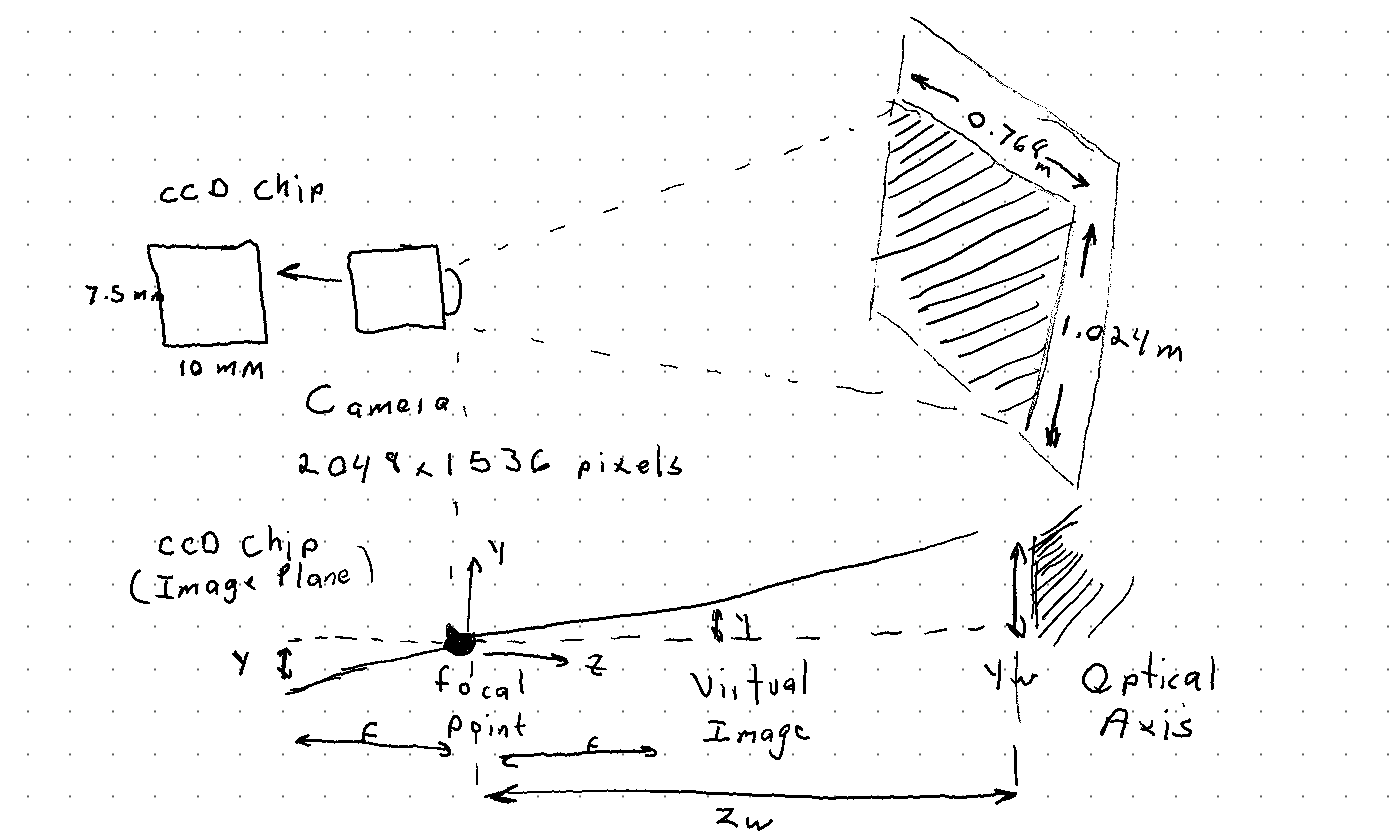
\includegraphics{./images/sketch.png}
\caption{Sketch Image}
\end{figure}

    \hypertarget{a-what-is-the-size-of-each-sensor-one-pixel-on-the-ccd-chip}{%
\subsubsection{a) What is the size of each sensor (one pixel) on the
CCD-Chip?}\label{a-what-is-the-size-of-each-sensor-one-pixel-on-the-ccd-chip}}

\[Scene_{Size}=1024mm \times 768mm\]
\[Camera_{resolution}=2048 \times 1536 \space pixels\]
\[CCD_{ActiveRegion}=10mm \times 7.5mm\]
\[Pixel_{sizeX}=\frac{10mm}{2048pixels}=0.0048mm=4.8 \mu m\]
\[Pixel_{sizeY}=\frac{7.5mm}{1536pixels}=0.0048mm=4.8 \mu m\]
\[Pixel_{Size}=4.8 \mu m \times 4.8 \mu m \]

    \hypertarget{b-what-is-the-scaling-coefficient-between-the-image-plane-ccd-chip-and-the-scene}{%
\subsubsection{b) What is the scaling coefficient between the image
plane (CCD-Chip) and the
scene?}\label{b-what-is-the-scaling-coefficient-between-the-image-plane-ccd-chip-and-the-scene}}

\[C_x=\frac{10mm}{1024mm}=0.97\]\\
\[C_y=\frac{7.5mm}{768mm}=0.97\] \textbf{The coefficient is 0.97 to 1 or
97 times smaller in the CCD-Chip than in the original scene}

\hypertarget{what-is-the-scaling-coefficient-between-the-scene-coordinates-and-the-image-pixels}{%
\subsubsection{What is the scaling coefficient between the scene
coordinates and the image
pixels?}\label{what-is-the-scaling-coefficient-between-the-scene-coordinates-and-the-image-pixels}}

\[C_x=\frac{1024}{2048}=0.5\]\\
\[C_y=\frac{768}{1536}=0.5\] \textbf{The coefficient is 1 to 1/2}

    \hypertarget{problem-3}{%
\subsection{Problem 3}\label{problem-3}}

Translation from the scene to a camera sensor can be done using a
transformation matrix, \(T\).

\begin{equation}
    \begin{bmatrix} x\\y\\1\end{bmatrix} = 
    T
    \begin{bmatrix}
        x_w\\ y_w\\ 1
    \end{bmatrix}\\
\end{equation} where \begin{equation}
    T= \begin{bmatrix} \alpha_x & 0 & x_0\\
            0 & \alpha_y & y_0\\
        0   & 0 & 1
    \end{bmatrix}
\end{equation} \(\alpha_x\) and \(\alpha_y\) are the scaling factors for
their corresponding axes.

Write a function in Python that computes the image points using the
transformation matrix, using the parameters from Problem 2. Let the
input to the function be a set of \(K\) scene points, given by a
\(2 \times K\) matrix, and the output the resulting image points also
given by a \(2 \times K\) matrix. The parameters defining the image
sensor and field of view from the camera center to the wall can also be
given as input parameters.

Test the function for the following input points given as a matrix:
\begin{equation}\label{cam-eq4}
    {\mathbf P}_{in} = \begin{bmatrix} 0.512 & -0.512 & -0.512 & 0.512 & 0 & 0.3 & 0.3 & 0.3 & 0.6 \\
    0.384 & 0.384 & -0.384 & -0.384 & 0 & 0.2 & -0.2 & -0.4 & 0 \end{bmatrix}.
\end{equation}

Comment on the results, especially notice the two last points!

    \begin{tcolorbox}[breakable, size=fbox, boxrule=1pt, pad at break*=1mm,colback=cellbackground, colframe=cellborder]
\prompt{In}{incolor}{2}{\boxspacing}
\begin{Verbatim}[commandchars=\\\{\}]
\PY{c+c1}{\PYZsh{} Import the packages that are useful inside the definition of the weakPerspective function}
\PY{k+kn}{import} \PY{n+nn}{math} 
\PY{k+kn}{import} \PY{n+nn}{numpy} \PY{k}{as} \PY{n+nn}{np}
\PY{k+kn}{import} \PY{n+nn}{matplotlib}\PY{n+nn}{.}\PY{n+nn}{pyplot} \PY{k}{as} \PY{n+nn}{plt}
\end{Verbatim}
\end{tcolorbox}

    \begin{tcolorbox}[breakable, size=fbox, boxrule=1pt, pad at break*=1mm,colback=cellbackground, colframe=cellborder]
\prompt{In}{incolor}{47}{\boxspacing}
\begin{Verbatim}[commandchars=\\\{\}]
\PY{l+s+sd}{\PYZdq{}\PYZdq{}\PYZdq{}}
\PY{l+s+sd}{Function that takes in input:}
\PY{l+s+sd}{\PYZhy{} FOV: field of view,}
\PY{l+s+sd}{\PYZhy{} sensorsize: size of the sensor,}
\PY{l+s+sd}{\PYZhy{} n\PYZus{}pixels: camera pixels,}
\PY{l+s+sd}{\PYZhy{} p\PYZus{}scene: K input points (2xK matrix)}

\PY{l+s+sd}{and return the resulting image points given the 2xK matrix}
\PY{l+s+sd}{\PYZdq{}\PYZdq{}\PYZdq{}}
\PY{k}{def} \PY{n+nf}{weakPerspective}\PY{p}{(}\PY{n}{FOV}\PY{p}{,} \PY{n}{sensorsize}\PY{p}{,} \PY{n}{n\PYZus{}pixels}\PY{p}{,} \PY{n}{p\PYZus{}scene}\PY{p}{)}\PY{p}{:}
    \PY{n}{scale\PYZus{}coefficient\PYZus{}scene} \PY{o}{=} \PY{n}{sensorsize}\PY{o}{/}\PY{n}{FOV}
    \PY{n}{scale\PYZus{}coefficient\PYZus{}sensor} \PY{o}{=} \PY{n}{FOV}\PY{o}{/}\PY{n}{n\PYZus{}pixels}
    
    \PY{n}{scale}\PY{o}{=} \PY{n}{scale\PYZus{}coefficient\PYZus{}scene} \PY{o}{*} \PY{n}{scale\PYZus{}coefficient\PYZus{}sensor}
    \PY{n}{p\PYZus{}scene} \PY{o}{=} \PY{n}{np}\PY{o}{.}\PY{n}{vstack}\PY{p}{(}\PY{p}{[}\PY{n}{p\PYZus{}scene}\PY{p}{,} \PY{n}{np}\PY{o}{.}\PY{n}{ones}\PY{p}{(}\PY{n}{p\PYZus{}scene}\PY{o}{.}\PY{n}{shape}\PY{p}{[}\PY{l+m+mi}{1}\PY{p}{]}\PY{p}{)}\PY{p}{]}\PY{p}{)}

    \PY{n}{T} \PY{o}{=} \PY{n}{np}\PY{o}{.}\PY{n}{array}\PY{p}{(}\PY{p}{[}\PY{p}{[}\PY{n}{scale}\PY{p}{[}\PY{l+m+mi}{0}\PY{p}{]}\PY{p}{,}\PY{l+m+mi}{0}\PY{p}{,}\PY{n}{FOV}\PY{p}{[}\PY{l+m+mi}{0}\PY{p}{]}\PY{p}{]}\PY{p}{,} \PY{p}{[}\PY{l+m+mi}{0}\PY{p}{,}\PY{n}{scale}\PY{p}{[}\PY{l+m+mi}{1}\PY{p}{]}\PY{p}{,}\PY{n}{FOV}\PY{p}{[}\PY{l+m+mi}{1}\PY{p}{]}\PY{p}{]}\PY{p}{,} \PY{p}{[}\PY{l+m+mi}{0}\PY{p}{,}\PY{l+m+mi}{0}\PY{p}{,}\PY{l+m+mi}{1}\PY{p}{]}\PY{p}{]}\PY{p}{)}
    
    \PY{n}{result} \PY{o}{=} \PY{n}{np}\PY{o}{.}\PY{n}{round}\PY{p}{(} \PY{n}{T} \PY{o}{@} \PY{n}{p\PYZus{}scene}\PY{p}{,}\PY{l+m+mi}{2}\PY{p}{)} 
    \PY{n}{result}\PY{o}{.}\PY{n}{dtype} \PY{o}{=} \PY{l+s+s1}{\PYZsq{}}\PY{l+s+s1}{float32}\PY{l+s+s1}{\PYZsq{}}
    \PY{k}{return}  \PY{n}{result}
    
\end{Verbatim}
\end{tcolorbox}

    \begin{tcolorbox}[breakable, size=fbox, boxrule=1pt, pad at break*=1mm,colback=cellbackground, colframe=cellborder]
\prompt{In}{incolor}{48}{\boxspacing}
\begin{Verbatim}[commandchars=\\\{\}]
\PY{c+c1}{\PYZsh{} The above function is then called using the following parameters:}

\PY{c+c1}{\PYZsh{} Parameters}
\PY{n}{FOV} \PY{o}{=} \PY{n}{np}\PY{o}{.}\PY{n}{array}\PY{p}{(}\PY{p}{[}\PY{l+m+mi}{1024}\PY{p}{,} \PY{l+m+mi}{768}\PY{p}{]}\PY{p}{)}  \PY{c+c1}{\PYZsh{}plane size giveninmilimiters}
\PY{n}{sensorsize} \PY{o}{=} \PY{n}{np}\PY{o}{.}\PY{n}{array}\PY{p}{(}\PY{p}{[}\PY{l+m+mi}{10}\PY{p}{,} \PY{l+m+mf}{7.5}\PY{p}{]}\PY{p}{)} \PY{c+c1}{\PYZsh{} CCD Sensor size}
\PY{n}{n\PYZus{}pixels} \PY{o}{=} \PY{n}{np}\PY{o}{.}\PY{n}{array}\PY{p}{(}\PY{p}{[}\PY{l+m+mi}{2048}\PY{p}{,} \PY{l+m+mi}{1536}\PY{p}{]}\PY{p}{)}
\PY{n}{p\PYZus{}scene\PYZus{}x} \PY{o}{=} \PY{p}{[}\PY{l+m+mf}{0.512}\PY{p}{,} \PY{o}{\PYZhy{}}\PY{l+m+mf}{0.512}\PY{p}{,} \PY{o}{\PYZhy{}}\PY{l+m+mf}{0.512}\PY{p}{,} \PY{l+m+mf}{0.512}\PY{p}{,} \PY{l+m+mi}{0}\PY{p}{,} \PY{l+m+mf}{0.3}\PY{p}{,} \PY{l+m+mf}{0.3}\PY{p}{,} \PY{l+m+mf}{0.3}\PY{p}{,} \PY{l+m+mf}{0.6}\PY{p}{]}
\PY{n}{p\PYZus{}scene\PYZus{}y} \PY{o}{=} \PY{p}{[}\PY{l+m+mf}{0.384}\PY{p}{,} \PY{l+m+mf}{0.384}\PY{p}{,} \PY{o}{\PYZhy{}}\PY{l+m+mf}{0.384}\PY{p}{,} \PY{o}{\PYZhy{}}\PY{l+m+mf}{0.384}\PY{p}{,} \PY{l+m+mi}{0}\PY{p}{,} \PY{l+m+mf}{0.2}\PY{p}{,} \PY{o}{\PYZhy{}}\PY{l+m+mf}{0.2}\PY{p}{,} \PY{o}{\PYZhy{}}\PY{l+m+mf}{0.4}\PY{p}{,} \PY{l+m+mi}{0}\PY{p}{]}
\end{Verbatim}
\end{tcolorbox}

    \begin{tcolorbox}[breakable, size=fbox, boxrule=1pt, pad at break*=1mm,colback=cellbackground, colframe=cellborder]
\prompt{In}{incolor}{49}{\boxspacing}
\begin{Verbatim}[commandchars=\\\{\}]
\PY{c+c1}{\PYZsh{}\PYZsh{}\PYZsh{}\PYZsh{}}
\PY{c+c1}{\PYZsh{} This cell is locked; it can be only be executed to see the results. }
\PY{c+c1}{\PYZsh{}\PYZsh{}\PYZsh{}\PYZsh{}}
\PY{c+c1}{\PYZsh{} Input data:}
\PY{n}{p\PYZus{}scene} \PY{o}{=} \PY{n}{np}\PY{o}{.}\PY{n}{array}\PY{p}{(}\PY{p}{[}\PY{n}{p\PYZus{}scene\PYZus{}x}\PY{p}{,} \PY{n}{p\PYZus{}scene\PYZus{}y}\PY{p}{]}\PY{p}{)}

\PY{c+c1}{\PYZsh{} Call to the weakPerspective() function }
\PY{n}{pimage} \PY{o}{=} \PY{n}{weakPerspective}\PY{p}{(}\PY{n}{FOV}\PY{p}{,} \PY{n}{sensorsize}\PY{p}{,} \PY{n}{n\PYZus{}pixels}\PY{p}{,} \PY{n}{p\PYZus{}scene}\PY{p}{)}

\PY{c+c1}{\PYZsh{} Result: }
\PY{n+nb}{print}\PY{p}{(}\PY{n}{pimage}\PY{p}{)}
\end{Verbatim}
\end{tcolorbox}

    \begin{Verbatim}[commandchars=\\\{\}]
[[0.    4.5   0.    4.5   0.    4.5   0.    4.5   0.    4.5   0.    4.5
  0.    4.5   0.    4.5   0.    4.5  ]
 [0.    4.25  0.    4.25  0.    4.25  0.    4.25  0.    4.25  0.    4.25
  0.    4.25  0.    4.25  0.    4.25 ]
 [0.    1.875 0.    1.875 0.    1.875 0.    1.875 0.    1.875 0.    1.875
  0.    1.875 0.    1.875 0.    1.875]]
    \end{Verbatim}

    \hypertarget{delivery-dead-line-on-canvas-12-09-2021-at-2359}{%
\subsubsection{Delivery (dead line) on CANVAS: 12-09-2021 at
23:59}\label{delivery-dead-line-on-canvas-12-09-2021-at-2359}}

    \hypertarget{contact}{%
\subsection{Contact}\label{contact}}

\hypertarget{course-teacher}{%
\subsubsection{Course teacher}\label{course-teacher}}

Professor Kjersti Engan, room E-431

E-mail: kjersti.engan@uis.no

\hypertarget{teaching-assistant}{%
\subsubsection{Teaching assistant}\label{teaching-assistant}}

Tomasetti Luca, room E-401

E-mail: luca.tomasetti@uis.no

    \hypertarget{references}{%
\subsection{References}\label{references}}

{[}1{]} S. Birchfeld, Image Processing and Analysis. Cengage Learning,
2016.

{[}2{]} I. Austvoll, ``Machine/robot vision part I,'' University of
Stavanger, 2018. Compendium, CANVAS.


    % Add a bibliography block to the postdoc
    
    
    \end{minipage}    
\end{document}
